

\documentclass[journal]{IEEEtran}

\usepackage{amsmath,amssymb,amsfonts}
\usepackage{bm}
\usepackage{graphicx}
\usepackage{cite}
\usepackage{algorithm}
\usepackage{algorithmic}

\begin{document}

\title{Score-Only Sparse Electrode Attacks on EEG Recognition via Sparse-Channel Search}

\author{Duc}

\maketitle

\begin{abstract}
Can a score-only adversary flip an EEG subject recognizer by controlling only a few complete electrode traces? Existing EEG attacks often use dense perturbations, white-box gradients, channel-time sparsity, or frequency-domain distortion, so they do not measure this acquisition-channel attack surface. We study a non-targeted sparse-channel attack in which the adversary observes class scores and perturbs complete electrode traces using bounded EEG-band waveforms. We propose sparse-channel search (SCS), a black-box attack that ranks EEG channels by their population leverage on the recognition margin and refines waveform coefficients using simultaneous perturbation stochastic approximation (SPSA), a gradient-free optimizer, under a peak-amplitude constraint. SCS treats the electrode trace, rather than the individual time sample, as the sparse attack unit. We evaluate attack success rate (ASR) and the first-success channel count $k^\star$, the first number of controlled electrode traces at which a clean-correct decision flips. On an HBN R1 subject-recognition sweep from 20 to 122 enrolled subjects, SCS achieves 95.31--100.00\% ASR while successful trials require only 2.54--3.67 channels on average. Even for the 122-subject recognizer, SCS reaches 97.54\% ASR with mean $k^\star=3.22$ and median $k^\star=2$. A BNCI2014\_001 reference comparison further shows that complete-channel EEG-band waveform control is substantially more effective than channel-time sparse variants in this setting. These results identify complete-electrode control as a strong score-only attack surface for EEG recognition.
\end{abstract}

\begin{IEEEkeywords}
EEG, adversarial attack, black-box, score-only, sparse channels, SPSA.
\end{IEEEkeywords}

% ============================================================
\section{Introduction}
% ============================================================

An EEG subject-recognition system receives a multichannel EEG trial and predicts which enrolled person produced it. Under normal sensing, the trial is recorded from multiple electrodes, preprocessed, and passed to a classifier. Clean accuracy and biometric equal-error rate (EER) tell us whether this recognizer works when the input is not manipulated.

An adversarial attack asks a different question. Instead of measuring normal recognition, it adds a small, carefully chosen change to the input so that the model predicts the wrong identity. The goal is not random noise. The goal is a structured perturbation that moves the model's decision while keeping the attacked signal close to the original EEG trial.

EEG changes the meaning of sparsity. In image attacks, a sparse perturbation often means changing a small number of pixels. In EEG, the physical sensing interface is divided into electrode channels. Perturbing a complete electrode trace is therefore more meaningful than perturbing isolated time samples, because a full trace corresponds to a sensor or acquisition path.

This paper studies a sparse-channel adversarial attack on EEG recognition. Here, sparse means that the attack changes only a few complete EEG channels. A low first-success channel count means that the recognizer's decision can be flipped after perturbing only a small part of the sensing interface.

We also study a score-only setting. Score-only means that the attacker cannot inspect model weights, gradients, or training data. The attacker can only submit an EEG trial and observe class scores, such as the confidence assigned to each enrolled subject identity. Together with channel sparsity, this gives the paper's question: can an adversary reliably flip EEG recognition with only a few complete electrode traces, and does this vulnerability persist as the number of enrolled identities increases?

EEG differs from images in one fundamental way: its meaningful structure is spectrotemporal rather than spatial. Each electrode records a superposition of neural oscillations at characteristic frequencies --- theta ($4$--$8$~Hz), alpha ($8$--$13$~Hz), and beta ($13$--$30$~Hz) --- sampled at a fixed rate to produce a discrete-time multichannel signal. Machine learning models trained on this signal, such as EEGConformer~\cite{song2022eegconformer}, learn to identify these oscillatory patterns and have demonstrated strong recognition performance in motor imagery, emotion, and authentication tasks.

This spectrotemporal structure shapes the attack design. An arbitrary dense noise signal may appear as a wideband artifact and can be weakened by standard EEG preprocessing. In the attack model studied here, the perturbation is therefore restricted to EEG-band waveforms and to a small number of complete electrode traces.

Existing EEG attacks expose important vulnerabilities, but they leave a gap for this setting. Dense attacks perturb many samples; white-box attacks assume gradients; sparse channel-time attacks modify individual time locations; and frequency-domain attacks usually report distortion or query efficiency rather than the number of complete acquisition channels required to flip a recognizer. The missing attack model is score-only, sparse in complete electrode traces, and constrained to EEG-band waveforms.

We propose sparse-channel search (SCS) for this attack model. Conceptually, SCS first asks which electrode channels are most useful for reducing the model's confidence in the clean predicted subject \emph{on average} across a probe set, fixing a single universal channel order; it then attacks each trial by perturbing channels in that order with a bounded EEG-band waveform using only score queries. Technically, this is implemented by population leverage ranking of channels followed by SPSA refinement of waveform coefficients under a peak-ratio constraint.

This paper makes three contributions:
\begin{itemize}
    \item Formulate a score-only sparse-electrode attack for EEG recognition, where the adversary perturbs complete electrode traces under a peak-amplitude constraint.
    \item Introduce SCS, a channel-waveform search that combines population leverage ranking of channels with SPSA refinement of bounded EEG-band waveform coefficients, and give a ranking-stability law (Claim~1) that predicts how many probe trials the ranking needs.
    \item Show on HBN R1 subject recognition that SCS flips decisions with high ASR while using only a few channels, and that this low first-success channel count persists from 20 to 122 enrolled subjects.
\end{itemize}

% ============================================================
\section{Related Work}
% ============================================================

\subsection{Dense EEG Adversarial Attacks}

EEG-based brain-computer interfaces and recognition systems have been shown to be vulnerable to adversarial manipulation~\cite{zhang2021tiny,wu2023adversarial}. Early EEG attacks and universal adversarial perturbations demonstrated that small perturbations spread across many samples can substantially degrade CNN-based EEG classifiers~\cite{liu2021uap}. These dense attacks establish vulnerability, but they do not test whether a decision can be flipped by controlling only a few electrodes.

\subsection{Sparse EEG Attacks}

Sparse EEG attacks reduce the perturbation support. SAGA selects channel-time locations and optimizes them with a PGD-style solver~\cite{feng2021saga}. This is close in spirit to SCS because both attacks exploit sparsity, but the sparse unit is different. SAGA sparsifies individual channel-time samples and assumes white-box gradients, whereas SCS perturbs complete electrode traces using only score queries.

\subsection{Black-Box EEG Attacks}

Black-box EEG attacks are important when model gradients and parameters are unavailable. Query-efficient attacks such as QELDBA target brainprint recognition using high-frequency perturbations and sparse sampling~\cite{qian2025qeldba}. These attacks emphasize query efficiency and distortion, while SCS emphasizes score-only control of complete electrode traces and reports the first-success channel count.

\subsection{Time-Frequency and Physically Constrained EEG Attacks}

Several EEG attacks use signal structure more explicitly. Adversarial filtering studies evasion and backdoor effects through filter manipulation~\cite{meng2024adversarialfilter}; physically constrained attacks model propagation over the scalp~\cite{wang2022physical}; and TFAttack exploits time-frequency structure for brainprint recognition~\cite{yi2024tfattack}. These methods show that EEG perturbations should respect signal structure, but they do not jointly combine score-only access, complete-channel sparsity, and EEG-band waveform search.

\subsection{Sparse Attacks in Vision}

Adversarial examples in vision showed that small structured perturbations can change high-performing neural networks~\cite{szegedy2014intriguing,goodfellow2015explaining}. Black-box attacks further showed that adversaries may need only output scores or labels rather than gradients~\cite{papernot2017practical,chen2017zoo}. Sparse vision attacks often count how many pixels or spatial coordinates are changed; adversarial-ML papers call this an $l_0$ constraint. They often also bound the largest perturbation value, called an $l_\infty$ constraint~\cite{croce2019sparse}. SCS adapts this sparse-attack logic to EEG by changing the sparse unit from a pixel or time sample to a complete electrode trace.

Table~\ref{tab:eeg_attack_landscape} summarizes the attack gap. The closest prior families are SAGA, because it is sparse, and QELDBA, because it targets black-box brainprint recognition. However, SAGA assumes gradients and sparsifies individual channel-time samples, while QELDBA optimizes query efficiency and distortion in the frequency domain.

\begin{table*}[t]
\centering
\caption{Representative EEG adversarial attacks and how their threat models differ from SCS. ``Score-only'' means the search uses classifier scores but not gradients or model parameters.}
\label{tab:eeg_attack_landscape}
\scriptsize
\setlength{\tabcolsep}{2pt}
\begin{tabular}{p{0.17\textwidth}p{0.15\textwidth}p{0.20\textwidth}p{0.20\textwidth}p{0.18\textwidth}}
\hline
Method & Access model & Perturbation unit & Main reported quantity & Gap relative to SCS \\
\hline
Dense EEG evasion / UAP~\cite{zhang2021tiny,liu2021uap} & White-box or transfer & All samples or a universal waveform & Accuracy drop / attack success & Does not restrict perturbations to a few electrodes \\
SAGA~\cite{feng2021saga} & White-box gradients & Sparse channel-time samples & Accuracy drop under sparse masks & Sparse, but not score-only and not complete-electrode control \\
Physically constrained BMI attack~\cite{wang2022physical} & White-box gradients & Physically modeled EEG perturbation & Attack success under physical constraints & Models physical propagation but not sparse score-only electrode control \\
Adversarial filtering~\cite{meng2024adversarialfilter} & Filter/signal-processing control & Adversarial filter & Evasion or backdoor success & Attacks filtering behavior rather than acquisition-channel control \\
TFAttack~\cite{yi2024tfattack} & White-box / gray-box & Time-frequency wavelet perturbation & ASR and perceptual distortion & Brainprint-relevant, but not score-only sparse-electrode control \\
QELDBA~\cite{qian2025qeldba} & Black-box queries & High-frequency perturbation with sparse sampling & Query efficiency, ASR, distortion & Black-box brainprint attack, but not complete-electrode control \\
SCS (ours) & Score-only queries & Complete electrode traces with EEG-band waveforms & ASR and first-success channel count $k^\star$ & Directly attacks complete electrode traces \\
\hline
\end{tabular}
\end{table*}

These works motivate the present attack, but none jointly considers score-only access, complete-channel sparsity, and EEG-band waveform search.

% ============================================================
\section{Threat Model and Attack Objective}
% ============================================================

We now turn the attack story into notation. The recognizer receives an EEG trial and returns a score for each enrolled identity. The attacker starts from the model's clean prediction and tries to make any other identity receive a higher score. This is a non-targeted attack: the attacker only needs the prediction to change, not to become a particular chosen subject.

The attacker is score-only. It can submit modified EEG trials and observe the output scores, but it does not know model parameters, gradients, architecture internals, or training data. The attack therefore cannot directly differentiate through the model. It must discover useful channels and waveform changes through repeated score queries.

The attacker is sparse at the channel level. It can add a bounded waveform to a small number of complete electrode traces before recognition. This models control over acquisition paths or digital input channels, not modification of the subject's neural activity or the classifier. The channel count is the attack sparsity cost: lower channel count means a more sparse attack.

Let $\mathcal{D}=\{(\mathbf{X}_i,y_i)\}_{i=1}^{N}$ be the EEG dataset of $N$ trials, where each trial $\mathbf{X}_i\in\mathbb{R}^{C\times T}$ has $C$ channels and $T$ time samples, $i\in[N]:=\{1,\ldots,N\}$, and carries a ground-truth identity label $y_i\in\{1,\ldots,K\}$ over the $K$ enrolled identities. A subject-recognition model returns class scores $f(\mathbf{X}_i)\in\mathbb{R}^{K}$, and the predicted identity is
\begin{equation}
\hat{y}(\mathbf{X}_i)=\arg\max_{j\in\{1,\ldots,K\}} f_j(\mathbf{X}_i).
\end{equation}
Ties in the argmax are broken by a fixed deterministic rule.
The attack targets one trial at a time, but every quantity we later average over the dataset must keep its trial index. We therefore index the per-trial objects by $i$: the clean predicted identity $y_0^i=\hat{y}(\mathbf{X}_i)$, the perturbation $\mathbf{E}_i$ chosen for trial $\mathbf{X}_i$, the support it activates, and the first-success count $k_i^\star$. We drop the index only for a per-trial \emph{operator} that does not depend on which trial it acts on --- the margin functional, the waveform parameterization, and the SPSA update --- and we restore it whenever a quantity is compared or averaged across trials (the population ranking of Section~\ref{sec:scs} and the attack metrics). The attack is non-targeted: it succeeds if the prediction changes from $y_0^i$ to any other identity. This objective does not require the attacker to know the true label; true labels are used only to restrict attacks to clean-correct trials and to report clean accuracy and EER.

The score margin of a trial under a candidate label is the operator
\begin{equation}
M(\mathbf{X},y)=f_{y}(\mathbf{X})-\max_{j\neq y} f_j(\mathbf{X}),
\label{eq:margin}
\end{equation}
defined for any $\mathbf{X}\in\mathbb{R}^{C\times T}$ and $y\in\{1,\ldots,K\}$. The clean decision on trial $i$ is stable while $M(\mathbf{X}_i,y_0^i)>0$, and the attack on trial $i$ succeeds once $M(\mathbf{X}_i+\mathbf{E}_i,y_0^i)$ becomes negative.

\subsection{Perturbation Unit and Amplitude Constraint}

Two constraints define the attack surface. The first is channel sparsity: the perturbation should touch only a few complete electrode traces. The second is amplitude: the injected waveform should remain bounded relative to the original EEG trial.

The perturbation $\mathbf{E}_i\in\mathbb{R}^{C\times T}$ chosen for trial $\mathbf{X}_i$ produces $\mathbf{X}_i^{\mathrm{adv}}=\mathbf{X}_i+\mathbf{E}_i$. The set of electrodes it touches is given by the support operator
\begin{equation}
\mathcal{S}(\mathbf{E})=\{c:\|\mathbf{E}_{c,:}\|_2>0\},
\end{equation}
applied to the chosen perturbation. The support is \emph{not} a set fixed in advance: $\mathcal{S}(\mathbf{E}_i)$ is whatever channels the trial-dependent solution $\mathbf{E}_i$ activates, and $|\mathcal{S}(\mathbf{E}_i)|$ is the channel-count attack cost on trial $i$. This is the EEG analogue of sparse $l_0$ image attacks~\cite{croce2019sparse}, but the counted unit is now a complete electrode trace rather than an individual pixel or time sample.

The attack must also keep the injected signal amplitude explicit. We therefore impose a peak-ratio constraint relative to each clean trial,
\begin{equation}
\|\mathbf{E}_i\|_{\infty}\leq r_{\max}\|\mathbf{X}_i\|_{\infty},
\label{eq:peak_ratio}
\end{equation}
where $r_{\max}$ is the allowed injected peak as a fraction of the trial peak. The $l_\infty$ notation means the largest absolute sample value of the perturbation. This expresses the amplitude budget in the units of the measured EEG signal, so the same constraint can be applied across trials with different absolute scales.

\subsection{Sparse-Channel Attack Objective}

The ideal sparse-channel attack objective is now straightforward: for each trial $\mathbf{X}_i$, find the perturbation that touches the fewest electrode traces while flipping the prediction,
\begin{equation}
\begin{aligned}
\min_{\mathbf{E}_i\in\mathbb{R}^{C\times T}} \quad
& |\mathcal{S}(\mathbf{E}_i)| \\
\mathrm{s.t.}\quad
& M(\mathbf{X}_i+\mathbf{E}_i,y_0^i)<0,\\
& \|\mathbf{E}_i\|_{\infty}\leq r_{\max}\|\mathbf{X}_i\|_{\infty}.
\end{aligned}
\label{eq:attack_problem}
\end{equation}
The minimizer $\mathbf{E}_i^\star$, and hence the support it activates, depend on the trial $\mathbf{X}_i$. This problem is combinatorial and nonconvex because it combines discrete channel support selection with continuous waveform optimization. SCS is a black-box heuristic for finding a successful low-channel perturbation; it does not certify the exact global minimum in~\eqref{eq:attack_problem}. A success at $k$ shows that $k$ complete electrode traces are sufficient for SCS to flip the decision. A failure within the tested budget $B$ does not prove that no lower-channel perturbation exists.

\subsection{Attack Metrics}

SCS does not commit to a support up front: it grows a \emph{nested} support one electrode per step, $\mathcal{S}^{(1)}\subset\mathcal{S}^{(2)}\subset\cdots$ with $|\mathcal{S}^{(k)}|=k$, refining the waveform after each addition. Let $\mathcal{A}_k(\mathbf{X}_i,y_0^i)$ denote the trial that SCS returns at budget $k$, i.e.\ using support $\mathcal{S}^{(k)}$ and its refined coefficients on trial $\mathbf{X}_i$. The first-success channel count of trial $i$ is the first budget at which the margin flips,
\begin{equation}
k_i^\star=\min\{k:M(\mathcal{A}_k(\mathbf{X}_i,y_0^i),y_0^i)<0\}.
\label{eq:first_success}
\end{equation}
The minimization in~\eqref{eq:first_success} is over the tested SCS budgets, not over all possible perturbations. When no budget up to the maximum $B$ succeeds, $k_i^\star$ is undefined and trial $i$ is counted unsuccessful at every prefix up to $B$. Over the set of successful trials $\mathcal{I}^\star\subseteq[N]$, we report attack success rate (ASR), attacked accuracy, the mean and median of $\{k_i^\star\}_{i\in\mathcal{I}^\star}$, and $K90$, $K95$, and $K100$, the smallest channel counts whose cumulative prefix ASR over all attacked clean-correct trials reaches 90\%, 95\%, and 100\%.

Clean recognition quality is reported separately through validation accuracy and biometric equal-error rate (EER), where EER is the verification point at which false-accept and false-reject rates match. These metrics prevent attack success on a weak recognizer from being mistaken for a strong adversarial result.

% ============================================================
\section{Sparse-Channel Search}
\label{sec:scs}
% ============================================================

SCS builds a sparse-channel attack in two stages: a one-time population channel ranking and a per-trial waveform refinement. Stage~1 estimates a population leverage score for each electrode over a probe set and fixes a single universal channel order; this ranking cost is amortized across all attacked trials and is the part we analyze (Claim~1). Stage~2 attacks each trial by adding electrodes in that fixed order and refining the injected waveform coefficients with SPSA, a gradient-free optimizer that estimates whether a waveform change helps by comparing scores from a small number of nearby query points. Separating ranking from refinement lets the channel order carry a stability guarantee while the waveform stays adapted to each trial.

\subsection{Waveform Parameterization}

Once a channel is selected, SCS still needs a waveform that changes the recognition margin without becoming an obvious artifact. We restrict each injected trace to a low-dimensional waveform basis indexed by $m$. Let $\{b_m(t)\}_{m=1}^{r}$ be $r$ candidate waveforms over the $T$ samples $t\in\{0,\ldots,T-1\}$ of a trial window, where $h(t)$ is a Hanning envelope and $f_s$ is the sampling rate. The basis combines three families. The first $r_{\mathrm{osc}}$ atoms are Hanning-tapered sinusoids,
\begin{equation}
\tilde{b}_m(t)=h(t)\cos\!\left(2\pi f_m t/f_s+p_m\right),
\qquad f_m\in[f_{\min},f_{\max}],
\label{eq:basis}
\end{equation}
with frequencies $f_m$ and phases $p_m$ spread deterministically over the EEG band $[f_{\min},f_{\max}]$. The next $r_{\mathrm{hat}}$ atoms are Hanning-tapered triangular bumps that capture slow localized structure,
\begin{equation}
\tilde{b}_m(t)=h(t)\,\max\!\left(1-\frac{|t/(T-1)-\mu_m|}{w},\,0\right),
\label{eq:basis_hat}
\end{equation}
with centers $\mu_m$ spread over $[0,1]$ and width $w$. The remaining $r_{\mathrm{trend}}$ atoms are Hanning-tapered polynomial trends,
\begin{equation}
\tilde{b}_m(t)=h(t)\left(s(t)^{\,d_m}-\overline{s^{\,d_m}}\right),
\quad s(t)=\tfrac{2t}{T-1}-1,
\label{eq:basis_trend}
\end{equation}
of degree $d_m\in\{0,1,\ldots\}$, mean-subtracted for $d_m>0$. Every atom is normalized to unit norm, $b_m=\tilde{b}_m/\|\tilde{b}_m\|_2$. The Hanning taper makes each atom start and end smoothly at zero, avoiding edge transients. We craft the waveform this way because EEG evidence is rhythmic and band-limited: the sinusoids represent controllable rhythms, while the bump and trend atoms absorb slowly varying residual structure that a pure-rhythm basis cannot cheaply represent. Figure~\ref{fig:oscillatory_atom_taper} illustrates the taper for a 10~Hz atom.

This design is different from simply adding perturbations to isolated time points. Point-level changes are useful for generic sparse adversarial attacks, but they are a poor fit for this EEG threat model: an isolated sample change has little interpretation as sensor control, can introduce sharp high-frequency artifacts, and forces the black-box search to choose among many channel-time coordinates. A complete-channel waveform instead matches the acquisition unit, stays inside the frequency range used by the recognizer, and reduces the black-box search to a small set of waveform coefficients on selected channels.

\begin{figure}[t]
\centering
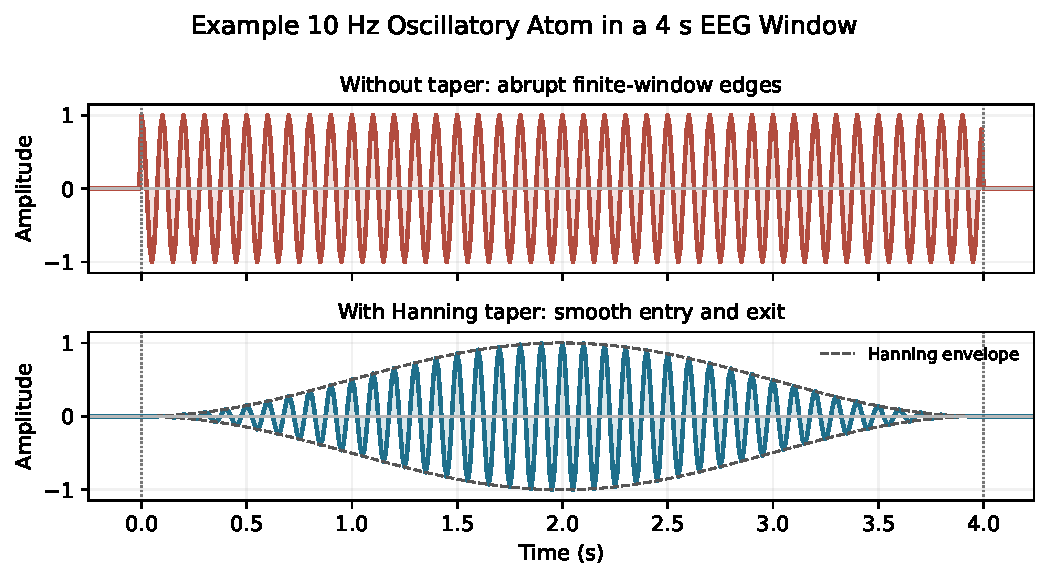
\includegraphics[width=\columnwidth]{Figure/oscillatory_atom_taper_example.pdf}
\caption{Example 10~Hz oscillatory atom over a 4-second HBN window. Without tapering, the finite-window cosine turns on and off abruptly at the segment boundaries. Multiplying by a Hanning window preserves the EEG-band oscillation while making the atom enter and exit smoothly, which is why SCS uses tapered atoms for waveform search.}
\label{fig:oscillatory_atom_taper}
\end{figure}

For a selected channel set $\mathcal{S}$, SCS stores one coefficient $a_{c,m}$ for each selected channel $c$ and basis waveform $b_m$. Let $\mathbf{A}\in\mathbb{R}^{C\times r}$ collect these coefficients, with rows outside $\mathcal{S}$ fixed to zero. The induced perturbation is
\begin{equation}
\left(\mathbf{E}_{\mathcal{S},\mathbf{A}}\right)_{c,t}=
\begin{cases}
\sum_{m=1}^{r} a_{c,m}b_m(t), & c\in\mathcal{S},\\
0, & c\notin\mathcal{S},
\end{cases}
\label{eq:parameterization}
\end{equation}
for each sample index $t$. The basis reduces the continuous search from all $C T$ samples to $|\mathcal{S}|r$ active coefficients.

\subsection{Score Objective}

SCS uses the margin in~\eqref{eq:margin} directly as its score-only objective. Reducing this margin means reducing the model's score advantage for the clean predicted identity. For a fixed support $\mathcal{S}$ and coefficients $\mathbf{A}$, the quantity evaluated by greedy probing and SPSA is
\begin{equation}
M(\mathbf{X}+\mathbf{E}_{\mathcal{S},\mathbf{A}},y_0).
\end{equation}
Success and the first-success channel count are evaluated using this same margin after enforcing the peak-ratio constraint in~\eqref{eq:peak_ratio}.

\subsection{Population Channel Ranking}

Channel selection is the part of the attack that decides which electrodes to control, and we want it to be both cheap (a one-time cost shared across all attacked trials) and analyzable. We therefore rank channels at the \emph{population} level: we estimate, for each electrode, how much controlling it reduces the recognition margin \emph{on average} over a set of probe trials, and we attack every trial by adding channels in that single fixed order.

\paragraph{Probe set and channel leverage.}
Let $\mathcal{D}_{\mathrm{probe}}\subseteq\mathcal{D}$ be a set of $n=|\mathcal{D}_{\mathrm{probe}}|$ probe trials, indexed by $i$, with clean predicted identity $y_0^i=\hat{y}(\mathbf{X}_i)$. This probe set need not be the model's training set. Let $\mathcal{P}=\{\mathbf{u}_1,\ldots,\mathbf{u}_{|\mathcal{P}|}\}$ be a fixed bank of sign vectors $\mathbf{u}\in\{-1,+1\}^{r}$. The \emph{leverage} of channel $c$ on trial $\mathbf{X}_i$ is the average single-channel margin drop produced by these probes,
\begin{equation}
g_c(\mathbf{X}_i)=M(\mathbf{X}_i,y_0^i)-\frac{1}{|\mathcal{P}|}\sum_{\mathbf{u}\in\mathcal{P}}M\!\left(\mathbf{X}_i+\mathbf{E}_{\{c\},\,\rho\,\mathbf{u}},\,y_0^i\right),
\label{eq:leverage}
\end{equation}
where $\rho$ is the probe amplitude and $\mathbf{E}_{\{c\},\rho\mathbf{u}}$ is the perturbation~\eqref{eq:parameterization} that places coefficients $\rho\mathbf{u}$ on channel $c$ alone, rescaled to satisfy~\eqref{eq:peak_ratio}. We use the \emph{average} drop, a sample statistic, rather than the best-case drop, so that the channel score is an empirical mean and the ranking is analyzable.

\paragraph{Population score and ranking.}
The population leverage of channel $c$ and its empirical estimate over the probe set are
\begin{equation}
L_c=\mathbb{E}_{\mathbf{X}}\!\left[g_c(\mathbf{X})\right],
\qquad
\widehat{L}_c=\frac{1}{n}\sum_{i=1}^{n} g_c(\mathbf{X}_i),
\label{eq:pop_leverage}
\end{equation}
where the expectation defining $L_c$ is over trials drawn from the same distribution as the dataset $\mathcal{D}$, and $\widehat{L}_c$ is its empirical mean over the $n$ probe trials. SCS ranks the $C$ channels by descending $\widehat{L}_c$, giving an empirical universal order $\widehat{\pi}=(\widehat{\pi}_1,\widehat{\pi}_2,\ldots,\widehat{\pi}_C)$ with $\widehat{L}_{\widehat{\pi}_1}\ge\widehat{L}_{\widehat{\pi}_2}\ge\cdots$. The nested support of Section~\ref{sec:scs} is then this fixed prefix, $\mathcal{S}^{(k)}=\{\widehat{\pi}_1,\ldots,\widehat{\pi}_k\}$, \emph{identical across trials}; only the refined coefficients (Section~\ref{subsec:spsa}) and the realized first-success count $k_i^\star$ depend on the trial $\mathbf{X}_i$. Thus $k_i^\star$ measures how far down the one universal order trial $i$ must go before its decision flips.

\paragraph{How many probes are enough?}
Ranking by an empirical mean is only trustworthy once $n$ is large enough that estimation noise cannot reorder channels that are truly separated. To state this precisely, let $\pi^\star=(\pi^\star_1,\ldots,\pi^\star_C)$ be the population order that sorts the true leverages, $L_{\pi^\star_1}\ge L_{\pi^\star_2}\ge\cdots$, and let $\widehat{\pi}$ be the empirical order used by SCS above. For a fixed budget $k<C$, assume the population frontier gap $\Delta=L_{\pi^\star_k}-L_{\pi^\star_{k+1}}$ is positive and that each per-trial leverage $g_c(\mathbf{X})$ is $\nu$-sub-Gaussian about its mean.

\medskip
\noindent\textbf{Claim~1 (channel-ranking stability).}
\emph{Fix $\delta\in(0,1)$ and a budget $k<C$. If the probe trials are drawn independently and
\begin{equation}
n\;\ge\;\frac{8\,\nu^2\,\log(2C/\delta)}{\Delta^2},
\label{eq:nstar}
\end{equation}
then with probability at least $1-\delta$ the empirical top-$k$ channel set used by SCS equals the population top-$k$ set, i.e., $\{\widehat{\pi}_1,\ldots,\widehat{\pi}_k\}=\{\pi^\star_1,\ldots,\pi^\star_k\}$.}

\medskip
\noindent\emph{Proof.}
(i)~If $\max_c|\widehat{L}_c-L_c|<\Delta/2$, then no two channels separated by at least $\Delta$ can swap order: for a pair with $L_a-L_b\ge\Delta$ we have $\widehat{L}_a>L_a-\Delta/2\ge L_b+\Delta/2>\widehat{L}_b$. Every (kept, dropped) pair across the frontier has population gap at least $\Delta$ by definition of $\Delta$, so no kept channel falls below a dropped one and the empirical top-$k$ set equals the population top-$k$ set. \emph{(proven, deterministic).}
(ii)~Each $\widehat{L}_c$ is a mean of $n$ independent $\nu$-sub-Gaussian terms, so $\Pr(|\widehat{L}_c-L_c|\ge\varepsilon)\le 2e^{-n\varepsilon^2/(2\nu^2)}$; a union bound over $C$ channels gives $\Pr(\max_c|\widehat{L}_c-L_c|\ge\varepsilon)\le 2C\,e^{-n\varepsilon^2/(2\nu^2)}$. \emph{(standard: sub-Gaussian tail + union bound).}
(iii)~Setting $\varepsilon=\Delta/2$ and the right-hand side to $\delta$ and solving for $n$ yields~\eqref{eq:nstar}. \emph{(proven).} \hfill$\square$

\medskip
The transferable content of Claim~1 is the \emph{form} of~\eqref{eq:nstar}, not the value of $n$: probe cost grows only as $\log C$ in the number of electrodes but as $1/\Delta^2$ in the frontier gap. Closely-ranked electrodes, not many electrodes, are what cost queries. The claim certifies stability of the channel order; it does not by itself prove that few channels will flip every trial. A low observed first-success count $k_i^\star$ has the separate interpretation that, once the order is stable, the early high-leverage electrodes are already sufficient to move the decision boundary for that trial.

We treat~\eqref{eq:nstar} as a prediction to be confirmed rather than a knob: we estimate $\nu$ from the empirical spread of $g_c$ across probe trials, estimate the empirical analogue of the frontier gap $\Delta$, and check that ranking agreement saturates near the predicted $n^\star$. Two assumptions are made explicit because the bound depends on them: probe trials are drawn independently --- realized by taking one window per distinct recording --- and $g_c$ is sub-Gaussian, which we verify empirically; if the leverage is heavy-tailed, a finite-variance (Bernstein) bound gives the same $1/\Delta^2$ rate with a larger constant.

\subsection{SPSA Refinement}
\label{subsec:spsa}

After each channel is added, the active coefficients are optimized using simultaneous perturbation stochastic approximation (SPSA)~\cite{spall1992spsa}. SPSA is a black-box optimization method: it randomly perturbs all active coefficients in positive and negative directions, checks how the score objective changes, and uses that difference to estimate a descent direction. It is appropriate here because SCS only observes classifier scores, yet each gradient estimate requires only two score queries regardless of the coefficient dimension.

Let $\mathbf{A}_\ell$ denote the current coefficient matrix, with rows outside $\mathcal{S}$ kept at zero. At iteration $\ell$, SPSA samples a random sign matrix $\mathbf{U}_\ell$ whose active rows contain $\{-1,+1\}$ entries and whose inactive rows are zero. With finite-difference radius $d_\ell$, it estimates a coefficient-gradient matrix
\begin{equation}
\widehat{\mathbf{G}}_\ell=
\frac{
\begin{aligned}
&M(\mathbf{X}+\mathbf{E}_{\mathcal{S},\mathbf{A}_\ell+d_\ell\mathbf{U}_\ell},y_0)\\
&{}-M(\mathbf{X}+\mathbf{E}_{\mathcal{S},\mathbf{A}_\ell-d_\ell\mathbf{U}_\ell},y_0)
\end{aligned}}
{2d_\ell}\mathbf{U}_\ell .
\label{eq:spsa_grad}
\end{equation}
The coefficients are updated as
\begin{equation}
\mathbf{A}_{\ell+1}
=\operatorname{Proj}\!\left(\mathbf{A}_\ell-q_\ell\widehat{\mathbf{G}}_\ell\right),
\label{eq:spsa_update}
\end{equation}
where $q_\ell$ is the SPSA step size and $\operatorname{Proj}(\cdot)$ keeps inactive rows at zero, clips the coefficient range, and rescales the synthesized perturbation if necessary to satisfy~\eqref{eq:peak_ratio}. Following standard SPSA gain schedules~\cite{spall1992spsa}, the finite-difference radius and step size decay as $d_\ell=d_0/(\ell+1)^{0.101}$ and $q_\ell=q_0/\sqrt{\ell+1}$. Multiple random restarts are used, and the best coefficient matrix under the query budget is retained.

The resulting procedure is summarized in Algorithm~\ref{alg:channel_sparse_attack}. It returns both the perturbed trial and the first tested support size at which the margin crosses zero. Low $k^\star$ means SCS changed the recognizer's decision by perturbing only a small number of complete electrode traces.

\begin{algorithm}[t]
\caption{Sparse-Channel Search (SCS)}
\label{alg:channel_sparse_attack}
\begin{algorithmic}[1]
\REQUIRE Probe set $\mathcal{D}_{\mathrm{probe}}$, test trial $\mathbf{X}$ with clean identity $y_0$, score oracle $f(\cdot)$, basis $\{b_m\}_{m=1}^{r}$, probe bank $\mathcal{P}$, probe amplitude $\rho$, channel budget $B$, peak ratio $r_{\max}$
\ENSURE Perturbed trial $\mathbf{X}^{\mathrm{adv}}$, first-success channel count $k^\star$

\STATE \textbf{Stage 1: population channel ranking (once for all trials)}
\FOR{each channel $c\in\{1,\ldots,C\}$}
    \STATE $\widehat{L}_c\leftarrow\frac{1}{n}\sum_{i=1}^{n} g_c(\mathbf{X}_i)$ over $\mathcal{D}_{\mathrm{probe}}$ using~\eqref{eq:leverage}
\ENDFOR
\STATE $\widehat{\pi}\leftarrow$ channels sorted by descending $\widehat{L}_c$
\STATE \textbf{Stage 2: per-trial attack in fixed order $\widehat{\pi}$}
\STATE $\mathcal{S}\leftarrow\varnothing$; initialize all active coefficients to zero
\FOR{$k=1$ \TO $B$}
    \STATE $\mathcal{S}\leftarrow\mathcal{S}\cup\{\widehat{\pi}_k\}$; warm-start the new row of $\mathbf{A}$ at zero
    \STATE Refine all coefficients on $\mathcal{S}$ by SPSA using~\eqref{eq:spsa_grad}--\eqref{eq:spsa_update}
    \STATE Rescale the synthesized perturbation to satisfy~\eqref{eq:peak_ratio}
    \IF{$M(\mathbf{X}+\mathbf{E}_{\mathcal{S},\mathbf{A}},y_0)<0$}
        \STATE $k^\star\leftarrow k$
        \STATE \textbf{return} $\mathbf{X}+\mathbf{E}_{\mathcal{S},\mathbf{A}}$, $k^\star$
    \ENDIF
\ENDFOR
\STATE \textbf{return} $\mathbf{X}+\mathbf{E}_{\mathcal{S},\mathbf{A}}$, failure within budget $B$
\end{algorithmic}
\end{algorithm}

% ============================================================
\section{Experimental Setup}
% ============================================================

The experimental question is whether the attack surface defined above remains strong as the number of enrolled HBN identities grows. We keep the assumptions fixed across the sweep: score-only non-targeted attacks on clean-correct trials, the same HBN release, the same 64-channel subset, the same passive-task/active-task split, and the same SCS configuration. The objective is therefore not to compare datasets, but to isolate whether low first-success channel counts persist under a larger identity set.

\subsection{Dataset, Model, and Preprocessing}

We use the Healthy Brain Network (HBN) R1-L100 EEG release and construct a subject-recognition task from eligible participants whose records contain both passive and active task recordings. Passive-task windows are used for training, and active-task windows are held out for validation. This split tests whether the recognizer learns subject-specific structure that transfers across task conditions rather than memorizing one recording condition.

\noindent\textbf{HBN R1-L100 setting.}
Subjects: 122 eligible participants in the largest sweep point, with nested subsets of 20, 35, 50, 75, and 100 subjects also evaluated. Recordings: 1,272 available EEG task recordings, split into 785 passive-task recordings for training and 487 active-task recordings for validation. EEG channels: 128-channel EGI GSN recordings, with a fixed 64-channel subset (E1--E64) used in all experiments. Sampling rate: 100~Hz in the BDF release and 100~Hz in the model input. Bandpass: 4--38~Hz. Windows: continuous recordings segmented into non-overlapping 4-second windows, giving 55,665 training windows and 44,694 validation windows at the 122-subject point. Window length: 4~s, corresponding to 400 samples per window.

Preprocessing keeps a fixed signal pipeline across the sweep: EEG channels are selected, scaled to microvolts, bandpass-filtered from 4--38~Hz, kept at 100~Hz, exponentially standardized, and windowed into non-overlapping 4-second segments. The main sweep uses nested subject sets of size $20$, $35$, $50$, $75$, $100$, and $122$. For every point in the sweep, the model sees the same fixed montage subset, channels E1--E64, so changes in the result are driven by the number of enrolled identities rather than by a changing channel surface. The primary recognizer is EEGConformer~\cite{song2022eegconformer}, trained with the same seed and preprocessing across the sweep.

\subsection{Attack Parameters}

After each clean model is trained, SCS is run on clean-correct validation trials with channel budget $B=12$, a 10\% peak-ratio cap, and 45,000 score calls per trial. We use $r=32$ atoms per selected channel: 16 oscillatory atoms spanning 2--30~Hz and 16 smooth residual/trend atoms. This gives SPSA 32 coefficients instead of all $T=400$ samples on a channel, balancing EEG-band expressiveness with black-box search cost. The attack sample count is at least 64 and grows with the subject count.

\subsection{Metrics and Baselines}

Clean recognition quality is reported by validation accuracy and pooled one-vs-rest EER. Attack effectiveness is reported by ASR, attacked accuracy on the attacked clean-correct trials, mean and median first-success channel count $k^\star$, and the prefix metrics $K90$, $K95$, and $K100$. The prefix metrics describe ASR as a function of channel budget: they are the smallest channel counts at which cumulative ASR reaches 90\%, 95\%, and 100\%. All HBN attacks use the same fixed query cap, so this paper reports channel-budget curves rather than an ASR-versus-query-budget sweep.

The main evidence is the HBN subject-count sweep. We also include a BNCI2014\_001 reference comparison against sparse channel-time variants to show why complete-electrode waveform control is the relevant perturbation unit for SCS.

% ============================================================
\section{Results}
% ============================================================

\subsection{Clean Recognition Under Subject Scaling} 

Before interpreting attack success, we first verify that the recognizer remains meaningful as the identity set grows. Table~\ref{tab:hbn_subject_sweep} shows the expected trend: as the enrolled set increases from 20 to 122 subjects, validation accuracy decreases from 96.55\% to 78.40\%, while pooled EER increases from 1.70\% to 4.10\%. The task is therefore becoming harder, but the 122-subject model is still far from a collapsed classifier.

This clean-recognition trend is important for attack interpretation. A high ASR on a weak model would not be informative; here, SCS is evaluated against recognizers that continue to separate subject identities with usable accuracy and low biometric EER.

\begin{table*}[t]
\centering
\caption{HBN R1 subject-count sweep for EEGConformer. All runs use 64 EEG channels, passive-task training, active-task validation, and the same SCS configuration. ASR is the fraction of clean-correct validation trials whose decision changes within the attack budget. Attacked accuracy is computed on the attacked clean-correct trials. Mean and median $k^\star$ are computed over successful attacks. A dash in $K100$ means SCS did not reach 100\% prefix ASR within the 12-channel budget.}
\label{tab:hbn_subject_sweep}
\scriptsize
\setlength{\tabcolsep}{2pt}
\begin{tabular}{rcccccccccc}
\hline
IDs & Acc. (\%) & EER (\%) & Attack trials & ASR (\%) & Att. acc. (\%) & Mean $k^\star$ & Med. $k^\star$ & $K90$ & $K95$ & $K100$ \\
\hline
20  & 96.55 & 1.70 & 64  & 98.44 & 1.56 & 2.54 & 2 & 6  & 8  & -- \\
35  & 93.95 & 1.85 & 64  & 95.31 & 4.69 & 3.59 & 3 & 11 & 12 & -- \\
50  & 91.77 & 2.17 & 64  & 100.00 & 0.00 & 3.67 & 3 & 8  & 9  & 12 \\
75  & 87.01 & 2.96 & 75  & 97.33 & 2.67 & 3.05 & 3 & 6  & 9  & -- \\
100 & 83.18 & 3.27 & 100 & 98.00 & 2.00 & 3.21 & 2 & 7  & 10 & -- \\
122 & 78.40 & 4.10 & 122 & 97.54 & 2.46 & 3.22 & 2 & 7  & 9  & -- \\
\hline
\end{tabular}
\end{table*}

\begin{figure*}[t]
\centering
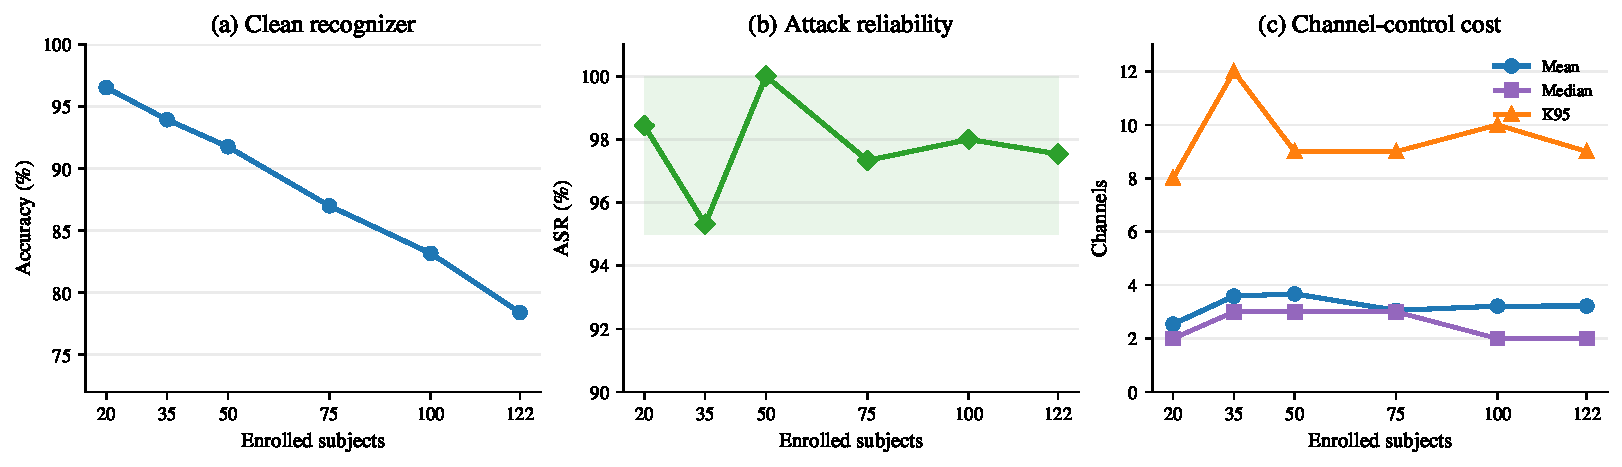
\includegraphics[width=0.98\textwidth]{Figure/hbn_scaling_dashboard.pdf}
\caption{Summary of the HBN subject-count sweep. As the enrolled identity set grows, clean recognition becomes harder: accuracy decreases and EER increases. SCS remains high-success, and the mean/median first-success channel count stays low.}
\label{fig:hbn_scaling_dashboard}
\end{figure*}

\subsection{SCS Remains Effective as Identities Increase}

Once the clean models are established, the central question is whether SCS remains effective as the subject set grows. Table~\ref{tab:hbn_subject_sweep} and Fig.~\ref{fig:hbn_scaling_dashboard} show persistent low-channel attack success across the sweep. Across all six subject counts, ASR remains between 95.31\% and 100.00\%, while the mean first-success channel count stays between 2.54 and 3.67 channels. Even at 122 subjects, SCS changes the decision on 97.54\% of attacked clean-correct trials, with a mean $k^\star$ of 3.22 channels and median $k^\star$ of 2 channels.

The tail of the distribution is also small. At 122 subjects, cumulative prefix ASR reaches 90\% by 7 controlled channels and 95\% by 9 controlled channels. Thus, although the recognizer faces a much larger identity set, most successful attacks still require only a small fraction of the 64 available EEG channels.

This behavior is consistent with the geometry of subject recognition in multichannel EEG. Adding more enrolled identities makes the clean classification problem harder, which is reflected by lower accuracy and higher EER, but subject-specific evidence can still remain concentrated in a few informative electrode traces. A non-targeted attack only needs to push the clean trial across a nearby decision boundary. SCS is designed for exactly this setting: the probe stage searches for channels with high leverage on the current margin, and the waveform basis then changes those channels in the same frequency range used by the recognizer.

\begin{figure*}[t]
\centering
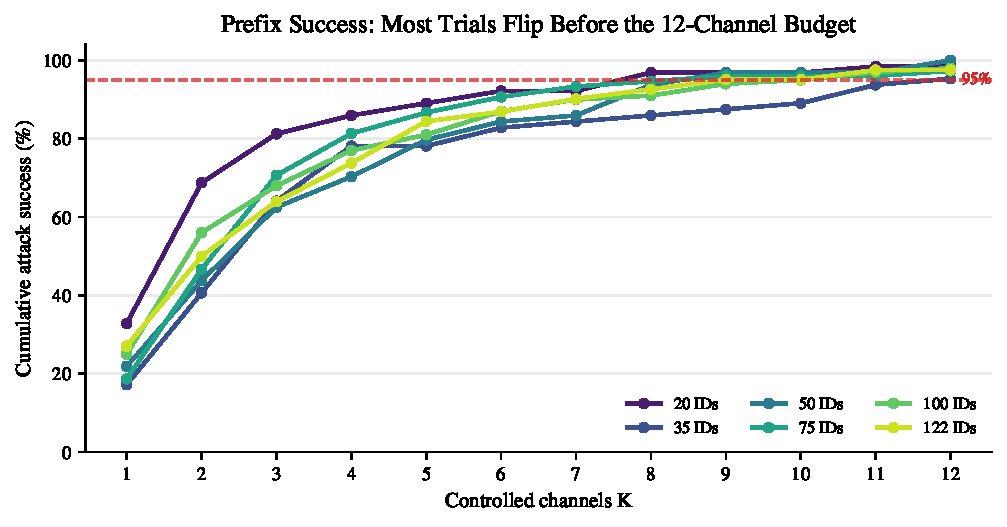
\includegraphics[width=0.82\textwidth]{Figure/hbn_prefix_success_curves.pdf}
\caption{Cumulative prefix ASR as the number of controlled channels increases. The curves show that successful attacks accumulate quickly for every subject-count setting, with most runs approaching or crossing 95\% ASR before the 12-channel budget.}
\label{fig:hbn_prefix_success}
\end{figure*}

Figure~\ref{fig:hbn_prefix_success} makes the channel-sparsity story more explicit. SCS does not rely on using all 12 allowed channels for most trials. Instead, the cumulative ASR curves rise sharply in the first few channels and then saturate near the final ASR.

The sharp early rise suggests that the first selected channels are not arbitrary. For many trials, they carry enough margin information that, once perturbed with a signal-consistent waveform, they determine whether the predicted identity remains stable. The later, slower part of each curve corresponds to harder trials whose clean margins are larger or whose discriminative evidence is spread across more channels.

\begin{figure*}[t]
\centering
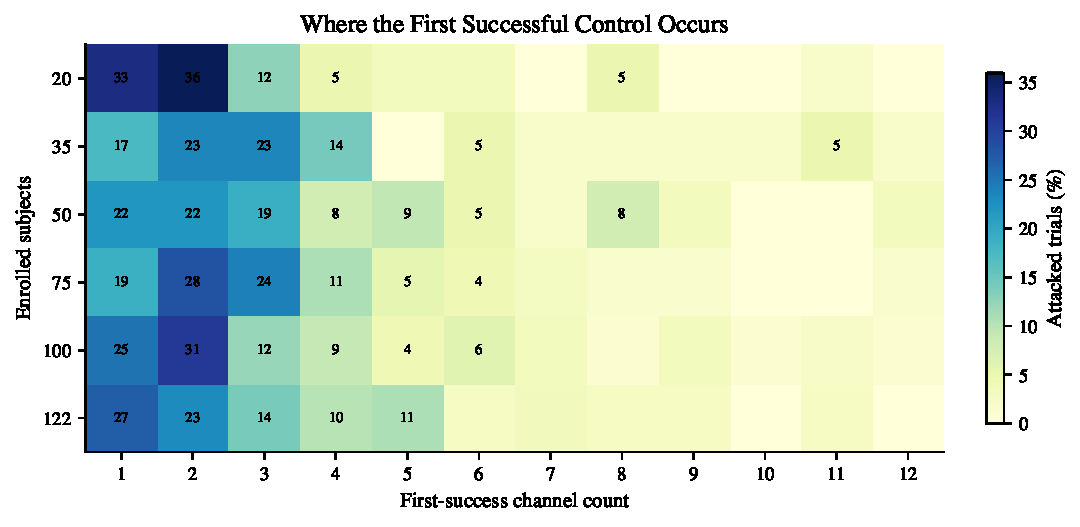
\includegraphics[width=0.82\textwidth]{Figure/hbn_first_success_heatmap.pdf}
\caption{Distribution of the first-success channel count. Each row sums the first-success attacks for one HBN subject-count run as a percentage of attacked clean-correct trials. The mass remains concentrated in the first few channels even for the 122-subject recognizer.}
\label{fig:hbn_first_success_heatmap}
\end{figure*}

The heatmap in Fig.~\ref{fig:hbn_first_success_heatmap} shows where the first successful attack occurs. Across the sweep, the largest cells are concentrated at one, two, and three channels. This view separates the typical case from the tail: SCS sometimes needs more channels, but the dominant behavior is sparse complete-electrode success.

The result supports persistence of low-channel attack success in this HBN sweep. It does not prove a universal law between subject count and adversarial robustness. With only six nested subject-count points, such a law would be too strong to claim. The supported claim is narrower and clearer: SCS remains effective from 20 to 122 enrolled subjects, and most successful attacks require only a few complete electrode traces.

\subsection{Reference Attack Comparison on BNCI2014\_001}

Published EEG attacks are not directly interchangeable baselines for the HBN sweep because they use different access assumptions, perturbation units, and success metrics. To make the attack-side comparison concrete, we also evaluate saved BNCI2014\_001 cross-session subject-recognition artifacts using the same EEGConformer checkpoint and the same 128 clean-correct validation windows. This reference setting has 9 subjects and 22 EEG channels, and all listed variants are capped at an 8-channel or channel-time budget where applicable.

\begin{table*}[t]
\centering
\caption{Reference attack comparison on BNCI2014\_001 subject recognition. The SAGA row is a paper-guided sparse channel-time PGD reconstruction included for comparison with a representative sparse EEG attack; it is not an official upstream implementation. Mean, median, and max $k^\star$ are computed over successful trials.}
\label{tab:bnci_attack_comparison}
\scriptsize
\begin{tabular}{p{0.27\textwidth}p{0.27\textwidth}ccccc}
\hline
Variant & Perturbation model & Trials & ASR (\%) & Attacked acc. (\%) & Mean $k^\star$ & Med. $k^\star$ \\
\hline
SCS: sparse channel + waveform & Score-only complete-channel waveform search & 128 & 72.66 & 27.34 & 3.47 & 3.0 \\
SAGA-style sparse channel-time PGD & Gradient-based sparse channel-time samples & 128 & 9.38 & 90.62 & 4.92 & 4.5 \\
Sparse channel-time + hybrid waveform & Score-only channel-time ablation with hybrid basis & 128 & 13.28 & 86.72 & 4.88 & 5.0 \\
\hline
\end{tabular}
\end{table*}

Table~\ref{tab:bnci_attack_comparison} supports the design choice behind SCS. In this subject-recognition setting, constraining the perturbation to local channel-time samples gives much lower success than allowing the attack to control complete electrode traces with smooth EEG-band waveforms. Thus, the waveform choice is not only a plausibility constraint; it also targets the perturbation unit that is effective for this recognizer. The comparison should be read as a reference attack study rather than a universal leaderboard: the main paper claim still comes from the HBN R1 sweep, while the BNCI comparison clarifies how the proposed perturbation unit differs from representative sparse EEG attack variants.

% ============================================================
\section{Discussion}
% ============================================================

The HBN sweep shows that complete-electrode traces are a strong sparse attack unit for EEG recognition. Accuracy and EER describe whether the recognizer separates subjects under clean sensing. They do not show whether a few acquisition channels are enough to flip a decision. In the 122-subject HBN setting, the recognizer still has usable clean performance, yet SCS changes most clean-correct decisions with only a few controlled traces.

The first implication is that sparse-channel EEG attacks should be evaluated at the level of complete electrode traces, not only channel-time samples. A single perturbed sample has little physical meaning, while a full channel trace corresponds to a sensor or acquisition path that can plausibly be corrupted. Measuring $k^\star$ therefore gives the attack an interpretable sparsity cost.

The second implication is that score-only access is enough to expose strong sparse-channel attack behavior in this setting. SCS does not require gradients or model parameters. Its probe stage ranks high-leverage channels from scores, and SPSA then refines waveform coefficients on the selected support.

The third implication is that increasing the number of enrolled identities does not eliminate the attack in the evaluated range. The clean task becomes harder as more subjects are enrolled, but SCS still reaches high ASR with low first-success channel counts. This is a persistence result, not a universal scaling law.

The fourth implication is that the perturbation model matters. A dense or wideband perturbation may overstate or mischaracterize the EEG threat because it ignores how EEG is acquired and filtered. The waveform basis and peak-ratio constraint keep SCS closer to EEG signal structure, so the low channel counts are not simply artifacts of unconstrained noise injection.

The main limitation is that the attack is evaluated digitally, not through hardware-in-the-loop signal injection. The HBN scaling study is also confined to Release 1 and uses six nested subject counts. Finally, SCS is a heuristic for the combinatorial objective in~\eqref{eq:attack_problem}; failure within the tested budget does not certify robustness. All HBN results use a fixed query cap, so a full ASR-versus-query-budget study remains future work.

% ============================================================
\section{Conclusion}
% ============================================================

We presented SCS, a score-only sparse-channel EEG attack that changes recognition decisions by perturbing a small number of complete electrode traces with bounded EEG-band waveforms. SCS combines greedy high-leverage channel selection with SPSA waveform refinement under a peak-ratio constraint, producing the per-trial first-success channel count $k^\star$. On the HBN R1 subject-recognition sweep, SCS remains high-success and low-channel from 20 to 122 enrolled subjects. These results show that complete-electrode waveform control is a strong adversarial surface for EEG recognition under score-only access.

\bibliographystyle{IEEEtran}
\bibliography{refs}

\end{document}
